\documentclass[english]{beamer}
\usepackage{makeidx}
\usepackage{color}
\usepackage{graphicx}
\usetheme{Goettingen}
\setbeamercovered{transparent}

\usenavigationsymbolstemplate{}
\AtBeginSection[]{
  \frame<beamer>{
    \frametitle{Next...}
    \tableofcontents[currentsection]
   }
}

\definecolor{ListingBorderColor}{gray}{0.55}
\definecolor{ListingBackgroundColor}{gray}{0.95}

\usepackage{babel}
\usepackage{hyperref}
\usepackage{enumerate}
\usepackage{enumerate}
\usepackage{longtable}
\usepackage[T1]{fontenc}
\usepackage{ucs}
\usepackage[latin1]{inputenc}
\usepackage{textcomp}
\usepackage{alltt}
\usepackage{listings}

\title{Git the basics}
\author{Bart Trojanowski, \href{mailto:bart@jukie.net}{bart@jukie.net}}
\institute{Jukie Networks Inc.}
\date{July 9th, 2008}

\setcounter{tocdepth}{1}


\newcommand{\mysection}[2]{
  \hypertarget{#2}{}
  \section{#1}
  \label{#2}
}
\newcommand{\mysubsection}[2]{
  \hypertarget{#2}{}
  \subsection{#1}
  \label{#2}
}

\definecolor{code-green}{rgb}{0,0.3,0}
\definecolor{code-orange}{rgb}{0.4,0.3,0}
\definecolor{code-blue}{rgb}{0,0,0.5}
\newcommand{\CMD}[1]{
  \texttt{\textcolor{code-green}{#1}}
}
\newcommand{\cmd}[1]{
  \texttt{\textcolor{code-orange}{#1}}
}
\newcommand{\gui}[1]{
  \texttt{\textcolor{code-blue}{#1}}
}


\begin{document}
% =====================================================================
\label{header}\hypertarget{header}{}
\frame{\maketitle}

% ---------------------------------------------------------------------
\begin{frame}
        \frametitle{Table of contents}
        \par\noindent
        \tableofcontents
\end{frame}

% =====================================================================
% =====================================================================
\mysection{Concepts}{_concepts}
% ---------------------------------------------------------------------
\begin{frame}
\frametitle{Concepts}
\begin{itemize}
        \item Source Control Management
                \begin{itemize}
                        \item track changes to files
                        \item repository / database of changes
                        \item working directory / current state
                \end{itemize}

        \pause{}
        \item Centralized SCM
                \begin{itemize}
                        \item server: single database
                        \item client: working directory \&{} state
                \end{itemize}

        \pause{}
        \item Decentralized SCM
                \begin{itemize}
                        \item anyone can be a server
                        \item repository coupled with working directory
                        \item complete history
                        \item disconnected operation
                \end{itemize}
\end{itemize}

\end{frame}

% =====================================================================
\mysubsection{SCM components}{_scm_components}

% ---------------------------------------------------------------------
\begin{frame}
\frametitle{SCM components}
\begin{columns}[t]
        \begin{column}{.5\textwidth}
                Working tree
                \begin{itemize}
                        \item directories
                        \item files
                \end{itemize}

        \end{column}
        \begin{column}[T]{.5\textwidth}
                \vspace{.2\textheight}
                \includegraphics[width=\linewidth]{repo-working-tree.eps}
        \end{column}
\end{columns}

\end{frame}

% ---------------------------------------------------------------------
\begin{frame}
\frametitle{SCM components}
\begin{columns}[t]
        \begin{column}{.5\textwidth}
                Repository contents
                \begin{itemize}
                        \item blobs
                \end{itemize}
        \end{column}
        \begin{column}[T]{.5\textwidth}
                \vspace{.2\textheight}
                \includegraphics[width=\linewidth]{repo-blob.eps}
        \end{column}
\end{columns}

\end{frame}

% ---------------------------------------------------------------------
\begin{frame}
\frametitle{SCM components}
\begin{columns}[t]
        \begin{column}{.5\textwidth}
                Repository contents
                \begin{itemize}
                        \item blobs
                        \item trees
                \end{itemize}
        \end{column}
        \begin{column}[T]{.5\textwidth}
                \vspace{.2\textheight}
                \includegraphics[width=\linewidth]{repo-tree.eps}
        \end{column}
\end{columns}

\end{frame}

% ---------------------------------------------------------------------
\begin{frame}
\frametitle{SCM components}
\begin{columns}[t]
        \begin{column}{.5\textwidth}
                Repository contents
                \begin{itemize}
                        \item blobs
                        \item trees
                        \item commits
                \end{itemize}
        \end{column}
        \begin{column}[T]{.5\textwidth}
                \vspace{.2\textheight}
                \includegraphics[width=\linewidth]{repo-commit.eps}
        \end{column}
\end{columns}

\end{frame}

% ---------------------------------------------------------------------
\begin{frame}
\frametitle{SCM components}
\begin{columns}[t]
        \begin{column}{.5\textwidth}
                Repository contents
                \begin{itemize}
                        \item blobs
                        \item trees
                        \item commits
                        \item ancestry
                \end{itemize}
        \end{column}
        \begin{column}[T]{.5\textwidth}
                \vspace{.2\textheight}
                \includegraphics[width=\linewidth]{repo-ancestry.eps}
        \end{column}
\end{columns}

\end{frame}

% ---------------------------------------------------------------------
\begin{frame}
\frametitle{SCM components}
\begin{columns}[t]
        \begin{column}{.5\textwidth}
                Repository contents
                \begin{itemize}
                        \item blobs
                        \item trees
                        \item commits
                        \item ancestry
                        \item tags
                \end{itemize}
        \end{column}
        \begin{column}[T]{.5\textwidth}
                \vspace{.2\textheight}
                \includegraphics[width=\linewidth]{repo-tags.eps}
        \end{column}
\end{columns}

\end{frame}

% ---------------------------------------------------------------------
\begin{frame}
\frametitle{SCM components}
\begin{columns}[t]
        \begin{column}{.5\textwidth}
                Repository contents
                \begin{itemize}
                        \item blobs
                        \item trees
                        \item commits
                        \item ancestry
                        \item tags
                        \item branches
                \end{itemize}
        \end{column}
        \begin{column}[T]{.5\textwidth}
                \vspace{.2\textheight}
                \includegraphics[width=\linewidth]{repo-branches.eps}
        \end{column}
\end{columns}

\end{frame}

% ---------------------------------------------------------------------
\begin{frame}
\frametitle{SCM components}
\begin{columns}[t]
        \begin{column}{.5\textwidth}
                HEAD
                \begin{itemize}
                        \item current checkout
                        \item points to branch
                        \item sometimes detached
                \end{itemize}
        \end{column}
        \begin{column}[T]{.5\textwidth}
                \vspace{.2\textheight}
                \includegraphics[width=\linewidth]{repo-head.eps}
        \end{column}
\end{columns}

\end{frame}

% ---------------------------------------------------------------------
\begin{frame}
\frametitle{SCM components}
\begin{columns}[t]
        \begin{column}{.5\textwidth}
                Index
                \begin{itemize}
                        \item ``staging area''
                        \item what is to be committed
                \end{itemize}
        \end{column}
        \begin{column}[T]{.5\textwidth}
                \vspace{.2\textheight}
                \includegraphics[width=\linewidth]{repo-index.eps}
        \end{column}
\end{columns}

\end{frame}

% =====================================================================
\mysubsection{SCM operations}{_scm_operations}

% ---------------------------------------------------------------------
\begin{frame}
\frametitle{SCM operations}
Bootstrap
\begin{itemize}
        \item init
        \item checkout
        \item switch branch
\end{itemize}

Modify
\begin{itemize}
        \item add, delete, rename
        \item commit
\end{itemize}

Information
\begin{itemize}
        \item status
        \item diff
        \item log
\end{itemize}

Reference
\begin{itemize}
        \item tag
        \item branch
\end{itemize}
\end{frame}

% ---------------------------------------------------------------------
\begin{frame}
\frametitle{Centralized SCM}
\includegraphics[width=\linewidth]{centralized.eps}
\begin{itemize}
        \item operations require \textcolor{red}{server}
                \begin{itemize}
                        \item single point of failure
                        \item bottleneck
                \end{itemize}
\end{itemize}
\end{frame}

% ---------------------------------------------------------------------
\begin{frame}
\frametitle{more SCM operations}
Decentralized
\begin{itemize}
        \item clone
        \item pull, fetch
        \item push
\end{itemize}
\end{frame}

% ---------------------------------------------------------------------
\begin{frame}
\frametitle{Decentralized SCM}
\includegraphics[width=\linewidth]{decentralized.eps}
\begin{itemize}
        \item anyone can be a server
\end{itemize}
\end{frame}

% =====================================================================
\mysubsection{Decentralization}{_decentralization}

% ---------------------------------------------------------------------
\begin{frame}
\frametitle{Decentralization}
\includegraphics[width=\linewidth]{cloning-1-upstream.eps}
\begin{itemize}
        \item public repository
\end{itemize}
\end{frame}

% ---------------------------------------------------------------------
\begin{frame}
\frametitle{Decentralization}
\includegraphics[width=\linewidth]{cloning-2-local.eps}
\begin{itemize}
        \item make a local clone
\end{itemize}
\end{frame}

% ---------------------------------------------------------------------
\begin{frame}
\frametitle{Decentralization}
\includegraphics[width=\linewidth]{cloning-3-topic.eps}
\begin{itemize}
        \item create topic ``branches''
\end{itemize}
\end{frame}

% ---------------------------------------------------------------------
\begin{frame}
\frametitle{Decentralization}
\includegraphics[width=\linewidth]{cloning-4-push.eps}
\begin{itemize}
        \item push changes between any repositories
\end{itemize}
\end{frame}

% ---------------------------------------------------------------------
\begin{frame}
\frametitle{Decentralization}
\includegraphics[width=\linewidth]{cloning-5-publish.eps}
\begin{itemize}
        \item publish changes to public server
\end{itemize}
\end{frame}

% ---------------------------------------------------------------------
\begin{frame}
\frametitle{Decentralization}
\includegraphics[width=\linewidth]{cloning-6-trusted.eps}
\begin{itemize}
        \item share changes with trusted peers
\end{itemize}
\end{frame}

% ---------------------------------------------------------------------
\begin{frame}
\frametitle{Is Decentralization any good?}

\begin{itemize}
        \item non-intrusive micro-commits
        \item detached operation
        \item no single point of failure
        \item backups are trivial
\end{itemize}
\end{frame}

% =====================================================================
% =====================================================================
\mysection{GIT History}{_git_history}
% ---------------------------------------------------------------------
\begin{frame}
\frametitle{Birth of GIT}
\begin{itemize}
        \item 2002
                \begin{itemize}
                        \item Linus uses BitKeeper for tracking Linux
                        \item BK gets better
                        \item Linux development scales better
                \end{itemize} 
        \pause{}
        \item April 6, 2005
                \begin{itemize}
                        \item BitMover drops free license
                        \item Linus writes his own SCM, GIT
                \end{itemize}
        \pause{}
        \item April 18, 2005
                \begin{itemize}
                        \item GIT can merge
                \end{itemize}
        \pause{}
        \item June 16, 2005
                \begin{itemize}
                        \item GIT is officially used to track Linux
                \end{itemize}
        \pause{}
        \item Feb 14, 2007
                \begin{itemize}
                        \item GIT 1.5.0 is released
                        \item major usability effort
                \end{itemize}
\end{itemize}
\end{frame}

% ---------------------------------------------------------------------
\begin{frame}
\frametitle{GIT gets better}

\begin{quote}
        And then realize that nothing is perfect.
        Git is just *closer* to perfect than any
        other SCM out there. \\
        -Linus
\end{quote}

\end{frame}

% =====================================================================
% =====================================================================
\mysection{Using GIT}{_using_git}
% ---------------------------------------------------------------------
\begin{frame}
\frametitle{Git commands}

\CMD{\$ git 
\textcolor{gray}{<options>}
<command>
\textcolor{gray}{<options>}}

\end{frame}

% ---------------------------------------------------------------------
\begin{frame}[fragile]
\frametitle{Git commands (137)}
{\tiny \tt
\begin{tabular}{llll}
add               & fast-export       & merge-one-file & revert             \\
am                & fast-import       & merge-resolve  & rm                 \\
annotate          & fetch             & merge-subtree  & send-email         \\
apply             & fetch-pack        & merge-tree     & send-pack          \\
archimport        & filter-branch     & mergetool      & sh-setup           \\
archive           & fmt-merge-msg     & mktag          & shell              \\
bisect            & for-each-ref      & mktree         & shortlog           \\
blame             & format-patch      & mv             & show               \\
branch            & fsck              & name-rev       & show-branch        \\
bundle            & fsck-objects      & pack-objects   & show-index         \\
cat-file          & gc                & pack-redundant & show-ref           \\
check-attr        & get-tar-commit-id & pack-refs      & stash              \\
check-ref-format  & grep              & parse-remote   & status             \\
checkout          & gui               & patch-id       & stripspace         \\
checkout-index    & hash-object       & peek-remote    & submodule          \\
cherry            & http-fetch        & prune          & svn                \\
cherry-pick       & http-push         & prune-packed   & symbolic-ref       \\
citool            & imap-send         & pull           & tag                \\
clean             & index-pack        & push           & tar-tree           \\
clone             & init              & quiltimport    & unpack-file        \\
commit            & init-db           & read-tree      & unpack-objects     \\
commit-tree       & instaweb          & rebase         & update-index       \\
config            & log               & receive-pack   & update-ref         \\
count-objects     & lost-found        & reflog         & update-server-info \\
cvsexportcommit   & ls-files          & relink         & upload-archive     \\
cvsimport         & ls-remote         & remote         & upload-pack        \\
cvsserver         & ls-tree           & repack         & var                \\
daemon            & mailinfo          & repo-config    & verify-pack        \\
describe          & mailsplit         & request-pull   & verify-tag         \\
diff              & merge             & rerere         & whatchanged        \\
diff-files        & merge-base        & reset          & write-tree         \\
diff-index        & merge-file        & rev-list       &                    \\
diff-tree         & merge-index       & rev-parse      &                    \\
\end{tabular}
}
\end{frame}

% ---------------------------------------------------------------------
\begin{frame}[fragile]
\frametitle{Git commands}
{\tiny \tt \textcolor{gray}{
\begin{tabular}{llll}
\CMD{add}              &      fast-export       &      merge-one-file & \cmd{revert}            \\
\cmd{am}               &      fast-import       &      merge-resolve  & \CMD{rm}                \\
\cmd{annotate}         & \CMD{fetch}            &      merge-subtree  & \cmd{send-email}        \\
\cmd{apply}            &      fetch-pack        &      merge-tree     &      send-pack          \\
     archimport        &      filter-branch     & \gui{mergetool}     &      sh-setup           \\
\cmd{archive}          &      fmt-merge-msg     &      mktag          & \gui{shell}             \\
\cmd{bisect}           &      for-each-ref      &      mktree         & \cmd{shortlog}          \\
\CMD{blame}            & \cmd{format-patch}     & \CMD{mv}            & \CMD{show}              \\
\CMD{branch}           &      fsck              &      name-rev       & \cmd{show-branch}       \\
\cmd{bundle}           &      fsck-objects      &      pack-objects   &      show-index         \\
     cat-file          & \CMD{gc}               &      pack-redundant &      show-ref           \\
     check-attr        &      get-tar-commit-id &      pack-refs      & \CMD{stash}             \\
     check-ref-format  & \CMD{grep}             &      parse-remote   & \CMD{status}            \\
\CMD{checkout}         & \gui{gui}              &      patch-id       &      stripspace         \\
     checkout-index    &      hash-object       &      peek-remote    & \CMD{submodule}         \\
\cmd{cherry}           &      http-fetch        &      prune          & \cmd{svn}               \\
\cmd{cherry-pick}      &      http-push         &      prune-packed   &      symbolic-ref       \\
\gui{citool}           &      imap-send         & \CMD{pull}          & \CMD{tag}               \\
\CMD{clean}            &      index-pack        & \CMD{push}          &      tar-tree           \\
\CMD{clone}            & \CMD{init}             & \cmd{quiltimport}   &      unpack-file        \\
\CMD{commit}           &      init-db           &      read-tree      &      unpack-objects     \\
     commit-tree       & \cmd{instaweb}         & \CMD{rebase}        &      update-index       \\
\CMD{config}           & \CMD{log}              &      receive-pack   &      update-ref         \\
     count-objects     &      lost-found        & \cmd{reflog}        & \cmd{update-server-info}\\
     cvsexportcommit   &      ls-files          &      relink         &      upload-archive     \\
     cvsimport         &      ls-remote         & \CMD{remote}        &      upload-pack        \\
     cvsserver         &      ls-tree           &      repack         &      var                \\
     daemon            &      mailinfo          &      repo-config    &      verify-pack        \\
\cmd{describe}         &      mailsplit         &      request-pull   &      verify-tag         \\
\CMD{diff}             & \CMD{merge}            &      rerere         & \cmd{whatchanged}       \\
     diff-files        &      merge-base        & \CMD{reset}         &      write-tree         \\
     diff-index        &      merge-file        &      rev-list       &                         \\
     diff-tree         &      merge-index       &      rev-parse      &                         \\
\end{tabular}
}}
\end{frame}

% ---------------------------------------------------------------------
\begin{frame}[fragile]
\frametitle{Git commands}
{\tiny
\CMD{\$ git help}
\begin{verbatim}
usage: git [--version] [--exec-path[=GIT_EXEC_PATH]] [-p|--paginate|--no-pager]
           [--bare] [--git-dir=GIT_DIR] [--work-tree=GIT_WORK_TREE] [--help]
           COMMAND [ARGS]

The most commonly used git commands are:
   add        Add file contents to the index
   bisect     Find the change that introduced a bug by binary search
   branch     List, create, or delete branches
   checkout   Checkout and switch to a branch
   clone      Clone a repository into a new directory
   commit     Record changes to the repository
   diff       Show changes between commits, commit and working tree, etc
   fetch      Download objects and refs from another repository
   grep       Print lines matching a pattern
   init       Create an empty git repository or reinitialize an existing one
   log        Show commit logs
   merge      Join two or more development histories together
   mv         Move or rename a file, a directory, or a symlink
   pull       Fetch from and merge with another repository or a local branch
   push       Update remote refs along with associated objects
   rebase     Forward-port local commits to the updated upstream head
   reset      Reset current HEAD to the specified state
   rm         Remove files from the working tree and from the index
   show       Show various types of objects
   status     Show the working tree status
   tag        Create, list, delete or verify a tag object signed with GPG
\end{verbatim}
}
\end{frame}

% ---------------------------------------------------------------------
\begin{frame}
\frametitle{Help}

\texttt{git <command> -h}
\begin{itemize}
        \item brief help output
\end{itemize}

\pause{}
\vspace{.1\textheight}

\texttt{man git-<command>}
\texttt{git help <command>}
\texttt{git <command> --help}
\begin{itemize}
        \item manual page
\end{itemize}

\end{frame}










% ---------------------------------------------------------------------
\begin{frame}
        END
\end{frame}

% =====================================================================
% vim: set makeprg=make:
\end{document}
